\documentclass{article}
\usepackage{amsmath}
\usepackage[legalpaper, margin=0.5in]{geometry}
\usepackage[final]{pdfpages}

\title{Exercises of Formal Languages and Automata Theory}
\author{Cecilia Chan}

\begin{document}
\maketitle

The problems are included at the end of the document.

\includepdf[pages=14]{Misc/Automata/200-only-problems.pdf}

\section*{Problem 1}
\subsection*{Part 1}
The fact that there exists at least one representation for the string $ w = v^1 $ where $ v = w $ is obvious. The challenge of this problem is to show that there is only one such representation such that $ v $ is primitive.

Thought process: As we always do, we assume there are two such representations and try to achieve a contradiction, and therefore I think $ a^m = b^n $ such that $ m \ne n $. For simplicity, let's us try $ m = 3 $ and $ n = 2 $. We get $ aaa = bb $, and for futher simplicity, we set $ a = "AB" $ and $ "b = "CDE" $, then $ "ABABAB" = "CDECDE" $, the individual character matches actually give us a lot of equalities. "A" = "C" = "E" = "D"  (just by checking the two rows must be the same, so C,E,D must be A) and "B" = "D" = "C" = "E", so in fact all letters are the same. That"s great because now we can claim that both $ a $ and $ b $ ar not primitive, so we have a contradiction we wanted. The key idea here is how do we generalize the above to any $ (m, n) $ pairs. To that end, I noticed the mod pattern and figured it out.

Suppose we compute $ g = \gcd(a, b) $ and therefore $ a = gp, b = gq, \gcd(p, q) = 1 $, we come up with a pattern similiar to above. Let $ a = a_0 a_1 \cdots a_{p-1} $ and $ b = b_0 b_1 \cdots b_{q-1} $ where each component has length $ g $. Now we can claim $ a_{x \mod p} = b_{x \mod q} $ , just like what we did above.

Thought process again: Now we wanted to show in fact all components are equal, so let's show any two pieces of $ a $ is in fact the same. In fact, that's enough because all we needed to show is one of the string is not primitive. So let's say we want to show $ a_i = a_j $, we know that it must go through some $ b_k $ since all we have above is equality between $ a_* $ and $ b_* $, how to I strategically find that $ k $. Turn out the equations are forcing us so.

\begin{eqnarray*}
  a_i = b_k &\implies& i \mod p = k \mod q \\
  b_k = a_j &\implies& k \mod q = j \mod p
\end{eqnarray*}

Rearranging, with additional arbitrary multipliers, we can have:
\begin{eqnarray*}
  i &=& k + \alpha p \\
  k &=& j + \beta q \\
  i &=& j + \beta q + \alpha p \\
  i - j &=& \beta q + \alpha p
\end{eqnarray*}

But remember that $ \gcd(p, q) = 1 $, so we can use Bezout's identity to find $ \alpha $ and $ \beta $ such that $ \alpha' p + \beta' q = 1 $, so multiplying both sides of this equation by $ (i - j) $, we will get what we wanted.

Of course, now we go back to the presentation of the proof, we claim that for any $ (i, j) $ pair such that  $ 0 \le i < j < p $. We have, by the Bezout identity, there exists $ \alpha' $ and $ \beta' $ such that:

\begin{eqnarray*}
  \alpha' p + \beta' q &=& 1 \\
  (j-i)\alpha' p + (j-i)\beta' q &=& (j-i) \\
  \alpha p + \beta q &=& j-i
\end{eqnarray*}

Now we can have:

\begin{eqnarray*}
  a_i &=& a_{(i + \alpha p) \mod p} \\
      &=& a_{(i + j-i - \beta q) \mod p} \\
      &=& a_{(j - \beta q) \mod p} \\
      &=& b_{(j - \beta q) \mod q} \\
      &=& b_{j \mod q} \\
      &=& a_{j \mod p} \\
      &=& a_j
\end{eqnarray*}

Now we reach a contradiction that $ a $ is in fact not primitive. This contradiction shows that the representation is unique and the concept of exponent is well defined.

\subsection*{Part 2}
To prove a relation is an equivalence relation, we need to show it is reflexive, symmetric and transitive. The first two are trivial, so we only need to show transitivity.

Suppose $ w_1 \sim w_2 $ and $ w_2 \sim w_3 $, we need to show $ w_1 \sim w_3 $. By definition, we can have $ a, b, p, q $ such that $ w_1 = ab $ , $ w_2 = ba = pq $ and $ w_3 = qp $.

Thought process: at this point, I must relate $ b $ and $ p $ somehow, but we don't know the relative lengths of $ b $ and $ p $, so we just do that case by case.

Case 1: $ |b| < |p| $, then we can write $ p = p_1 p_2 $ such that $ |p_1| = |b| $, now we have $ b = p_1 $ and $ a = p_2 q $, so $ w_1 = p_2 q p_1  $ and $ w_3 = q p_1 p_2 $, so $ w_1 \sim w_3 $

Case 2: $ |b| > |p| $, then we can write $ b = b_1 b_2 $ such that $ |b_1| = |p| $, now we have $ p = b_1 $ and $ q = b_2 a $, so $ w_3 = b_2 a b_1 $ and $ w_1 = a b_1 b_2 $, so $ w_3 \sim w_1 $, and by symmetry, $ w_1 \sim w_3 $.

Case 3: $ |b| = |p| $, then we can write $ b = p $ and $ a = q $, now we have $ w_1 = q p $ and $ w_3 = q p $, so $ w_1 \sim w_3 $.

In all case, we have shown that $ w_1 \sim w_3 $, so we have proved that the relation is transitive.

Thought process: through the exercise above we notice that conjugation is really just rotating, so let's see what would happen if we rotate. If we rotate by $ n $ position, we can do that by rotating it $ 1 $ letter at a time $ n $ times. If we could show that rotating one letter is fine, rotating by any number of letters will just be fine. So let's learn more about rotating strings by just one charcter.

Suppose we rotating a string $ v^n $ where $ |v| = 1 $, this is a trivial case since it will be the same.
Suppose we rotating a string $ v^n $ where $ |v| > 1 $, now we can let $ v = (a+b) $, and so the rotated string will be $ b(a+b)^{n-1}a $, but if we look closely, this is simply $ (b+a)^n $, we just need to parenthesize it differently. 

We can unify the both cases and say that if we rotate a string by one character, it is the same as rotating the primitive part and keep the exponent unchanged. Note that the result above holds even when $ n = 1 $. Immediately, we know this must be true for an arbitrary number of rotations, because we can just rotate one character at a time.

Now we can use this fact to argue rotating a string keep the exponent unchanged, suppose $ w = v^n $, rotating is simply rotating $ v $ and keep the exponent unchanged, so $ w' = v'^n $, Now $ w' $ must be primitive, because otherwise we can rotate backwards and show $ w $ is not primitive. So rotating doesn't change the exponent, all conjugates share the same exponent.

Thought process - one last step, the size of the equivalence class. I wanted to claim the size of the equivalence class is simply the length of the primitive part, so we need to prove that rotations of a primitive part are unique strings. Let's see what happen if it isn't.

Suppose $ v $ is primitive and $ v = p + q = q + p $, now we have the problem that we have seen in part 1, $ v $ cannot be primitive. So we have proved that rotations of a primitive part are unique strings.

With that, we can claim that the size of the equivalence class is simply the length of the primitive part.

\includepdf[pages=15]{Misc/Automata/200-only-problems.pdf}

\section*{Problem 2}
TODO

\section*{Problem 3}
TODO


\end{document}